%% Bookheader, Nov 8, 2020; July 18, 2022

\documentclass[11pt]{../Support/ourbook}
%% or for landscape, comment out line above and use this one:
%%\documentclass[landscape,11pt]{ourbook}

%% This will keep space from stretching around display math:

\makeatletter
\renewcommand\normalsize{%
   \@setfontsize\normalsize\@xipt{13.6}%
   \abovedisplayskip 11\p@  \@minus6\p@
   \abovedisplayshortskip \z@ 
   \belowdisplayshortskip 6.5\p@ \@minus3\p@
   \belowdisplayskip \abovedisplayskip
   \let\@listi\@listI}
\makeatother
\normalsize


\begin{document}

\tableofcontents
\graphicspath{{../../Chapters/matplotlib/en_US}}
\chapter{Making Plots with matplotlib}

Matplotlib is a comprehensive library for creating static, animated,
and interactive visualizations in Python. It's highly useful for
presenting data in a more intuitive and easy-to-understand manner.\index{matplotlib}

In order to use Matplotlib, you must first import it, typically using
the following line of code:

\begin{lstlisting}[language=Python]
import matplotlib.pyplot as plt
\end{lstlisting}

Let's create a simple line plot. Suppose we have a list of numbers and
we want to visualize their distribution:

\begin{lstlisting}[language=Python]
x = [1, 2, 3, 4, 5]
y = [1, 4, 9, 16, 25]

plt.plot(x, y)
plt.show()
\end{lstlisting}

Here, `x` and `y` are the coordinates of the points. The `plt.plot`
function plots y versus x as lines and/or markers. The `plt.show`
function then displays the figure.

Creating a bar plot follows a similar approach:

\begin{lstlisting}[language=Python]
labels = ['A', 'B', 'C', 'D', 'E']
values = [5, 7, 9, 11, 13]

plt.bar(labels, values)
plt.show()
\end{lstlisting}

Here, `labels` are the categories we are plotting, and `values` are
the respective sizes of those categories. The `plt.bar` function
creates a bar plot.

Matplotlib provides a variety of other plot types and customization
options - everything from scatter plots and histograms to custom line
styles and colors. Explore the official Matplotlib documentation to
learn more about what this powerful library can offer.

\graphicspath{{../../Chapters/geographical_data/en_US}}
\chapter{Geographical Data}


\graphicspath{{../../Chapters/long_lat_dist/en_US}}
\chapter{Longitude and Latitude}

\section{Longitude and Latitude}
The Earth can be represented as a sphere, and the position of a point
on its surface can be described using two coordinates: latitude and
longitude.

\begin{figure}[htbp]
    \centering
    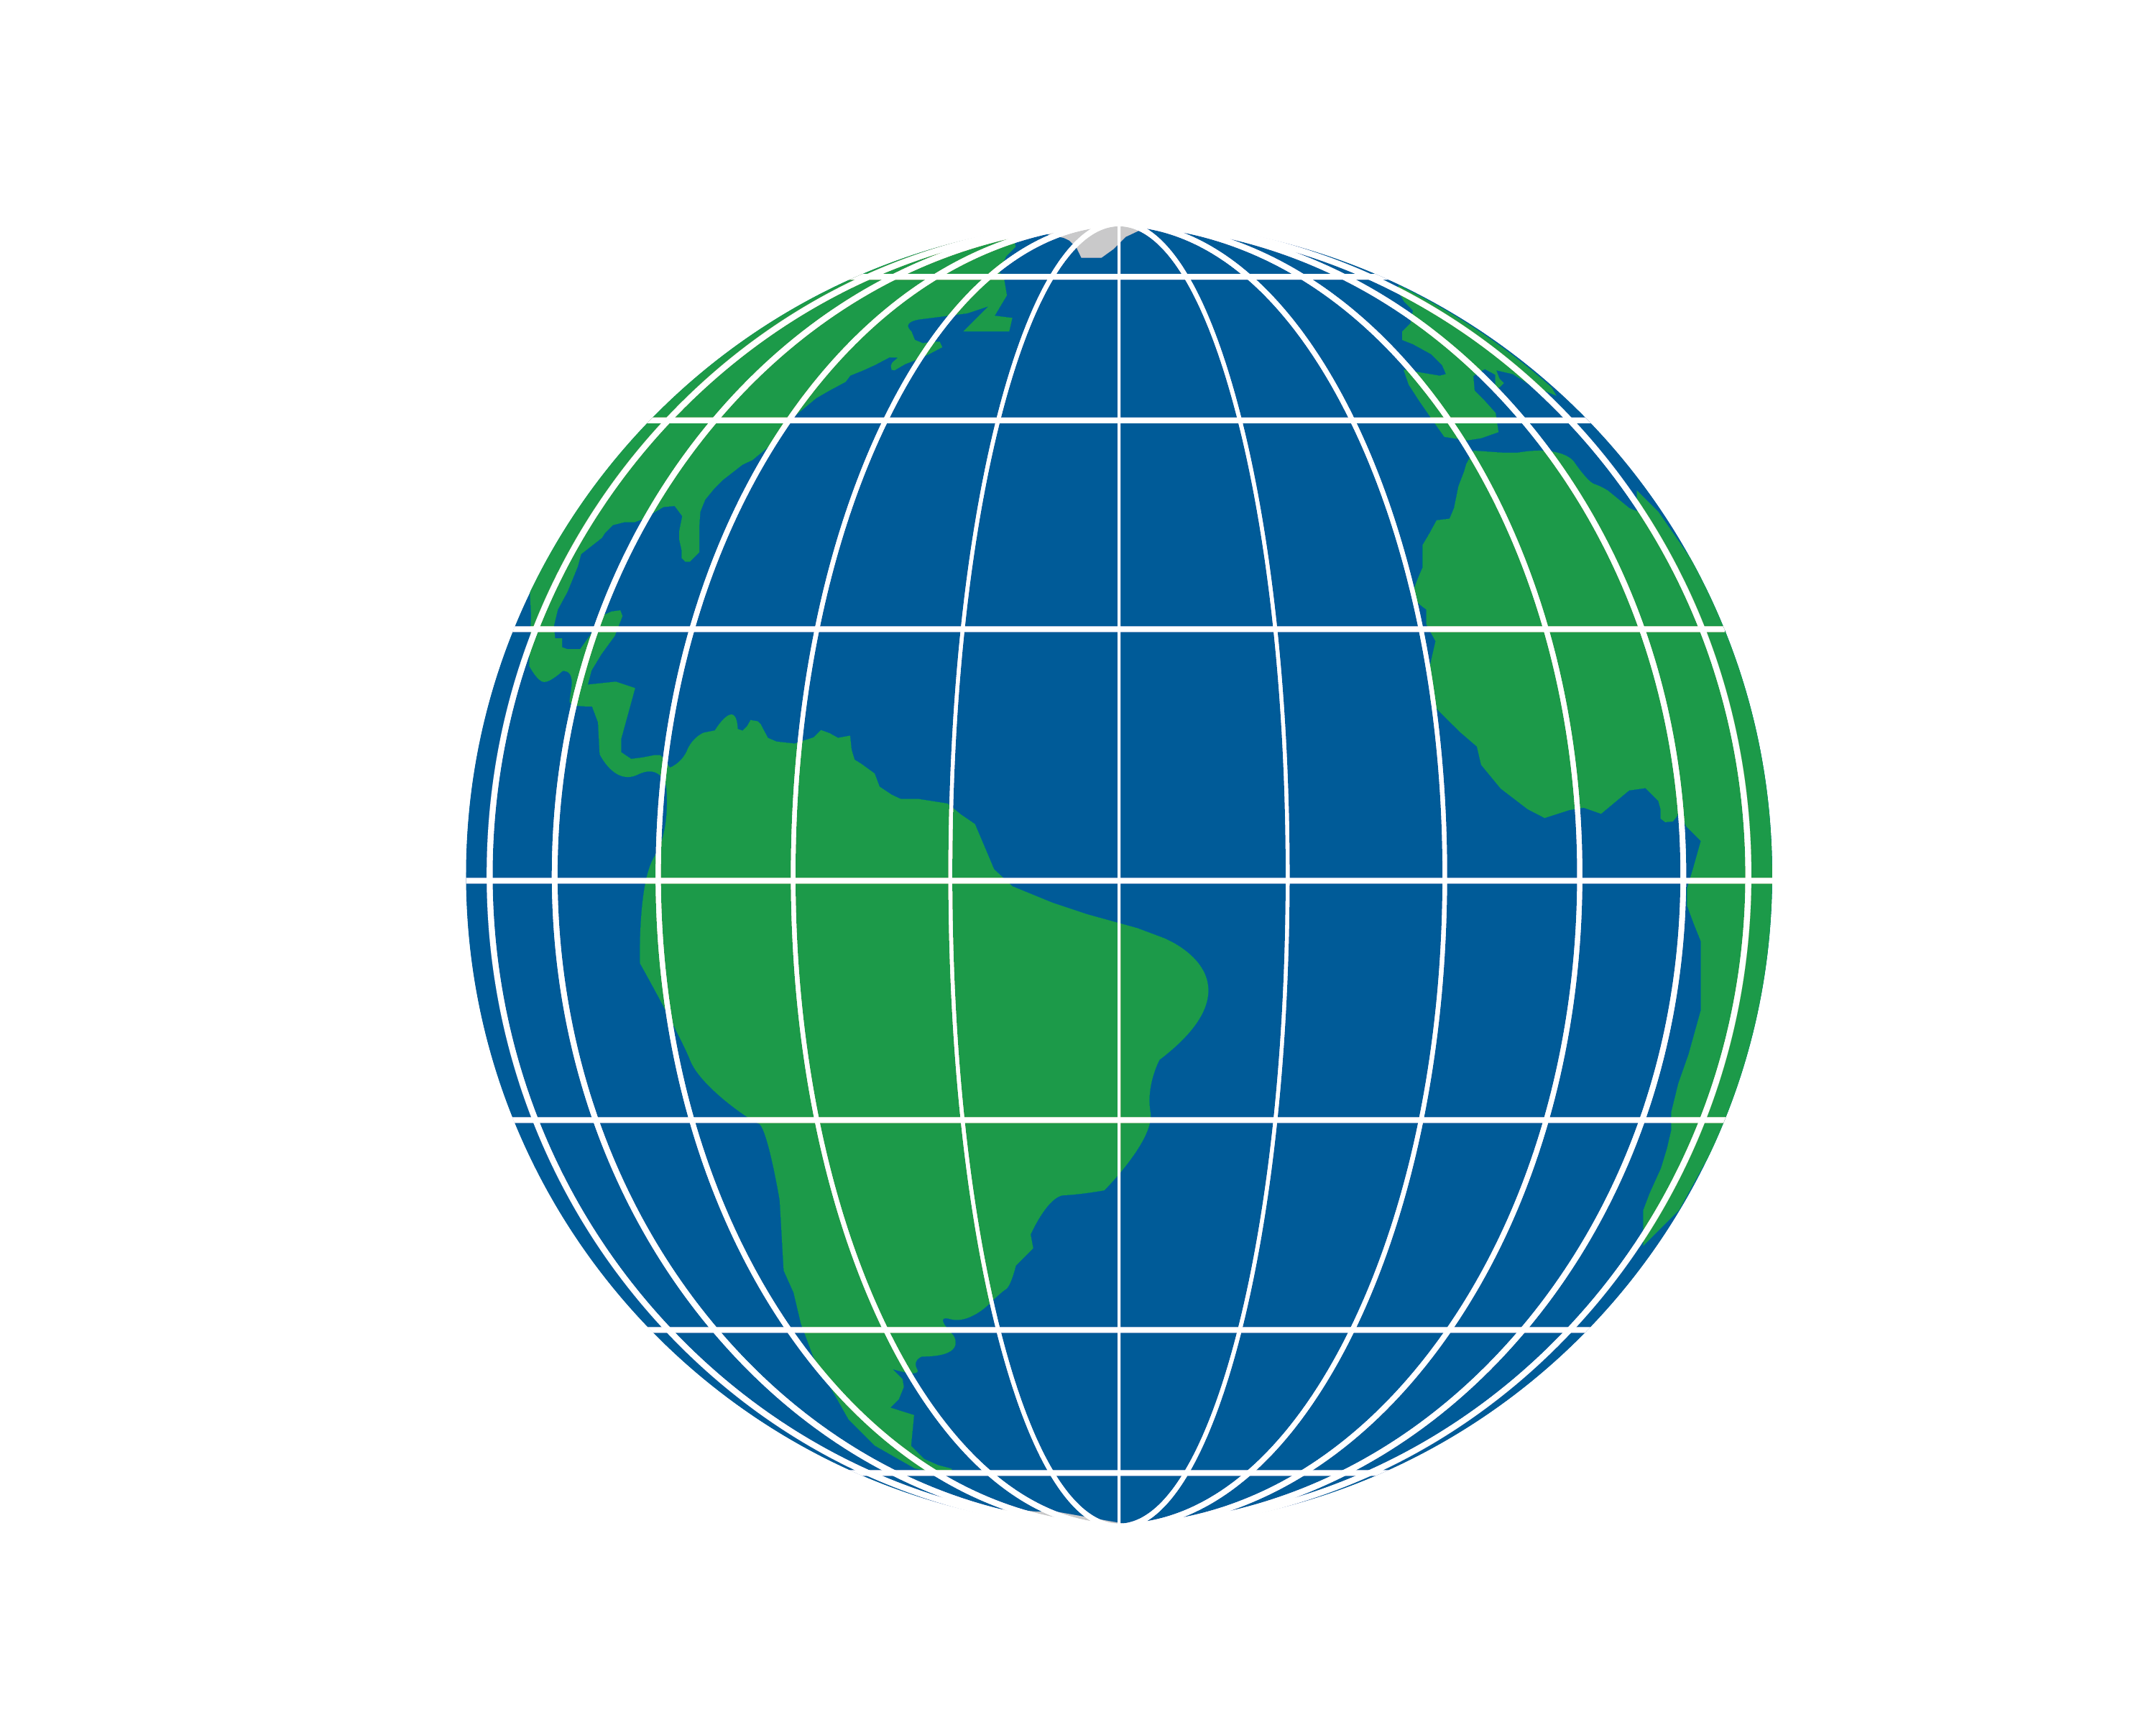
\includegraphics[width=.75\textwidth]{latLon.png}
    \caption{A diagram of latitude and longitude.}
    \label{fig:latLon}
\end{figure}

\index{latitude}
Latitude is a measure of a point's distance north or south of the
equator, expressed in degrees. It ranges from $-90^{\circ}$ at the
South Pole to $+90^{\circ}$ at the North Pole, with $0^{\circ}$
representing the Equator. (See figures~\ref{fig:latitude} and~\ref{fig:latitudeExplained})
\begin{figure}[htbp]
  \centering
  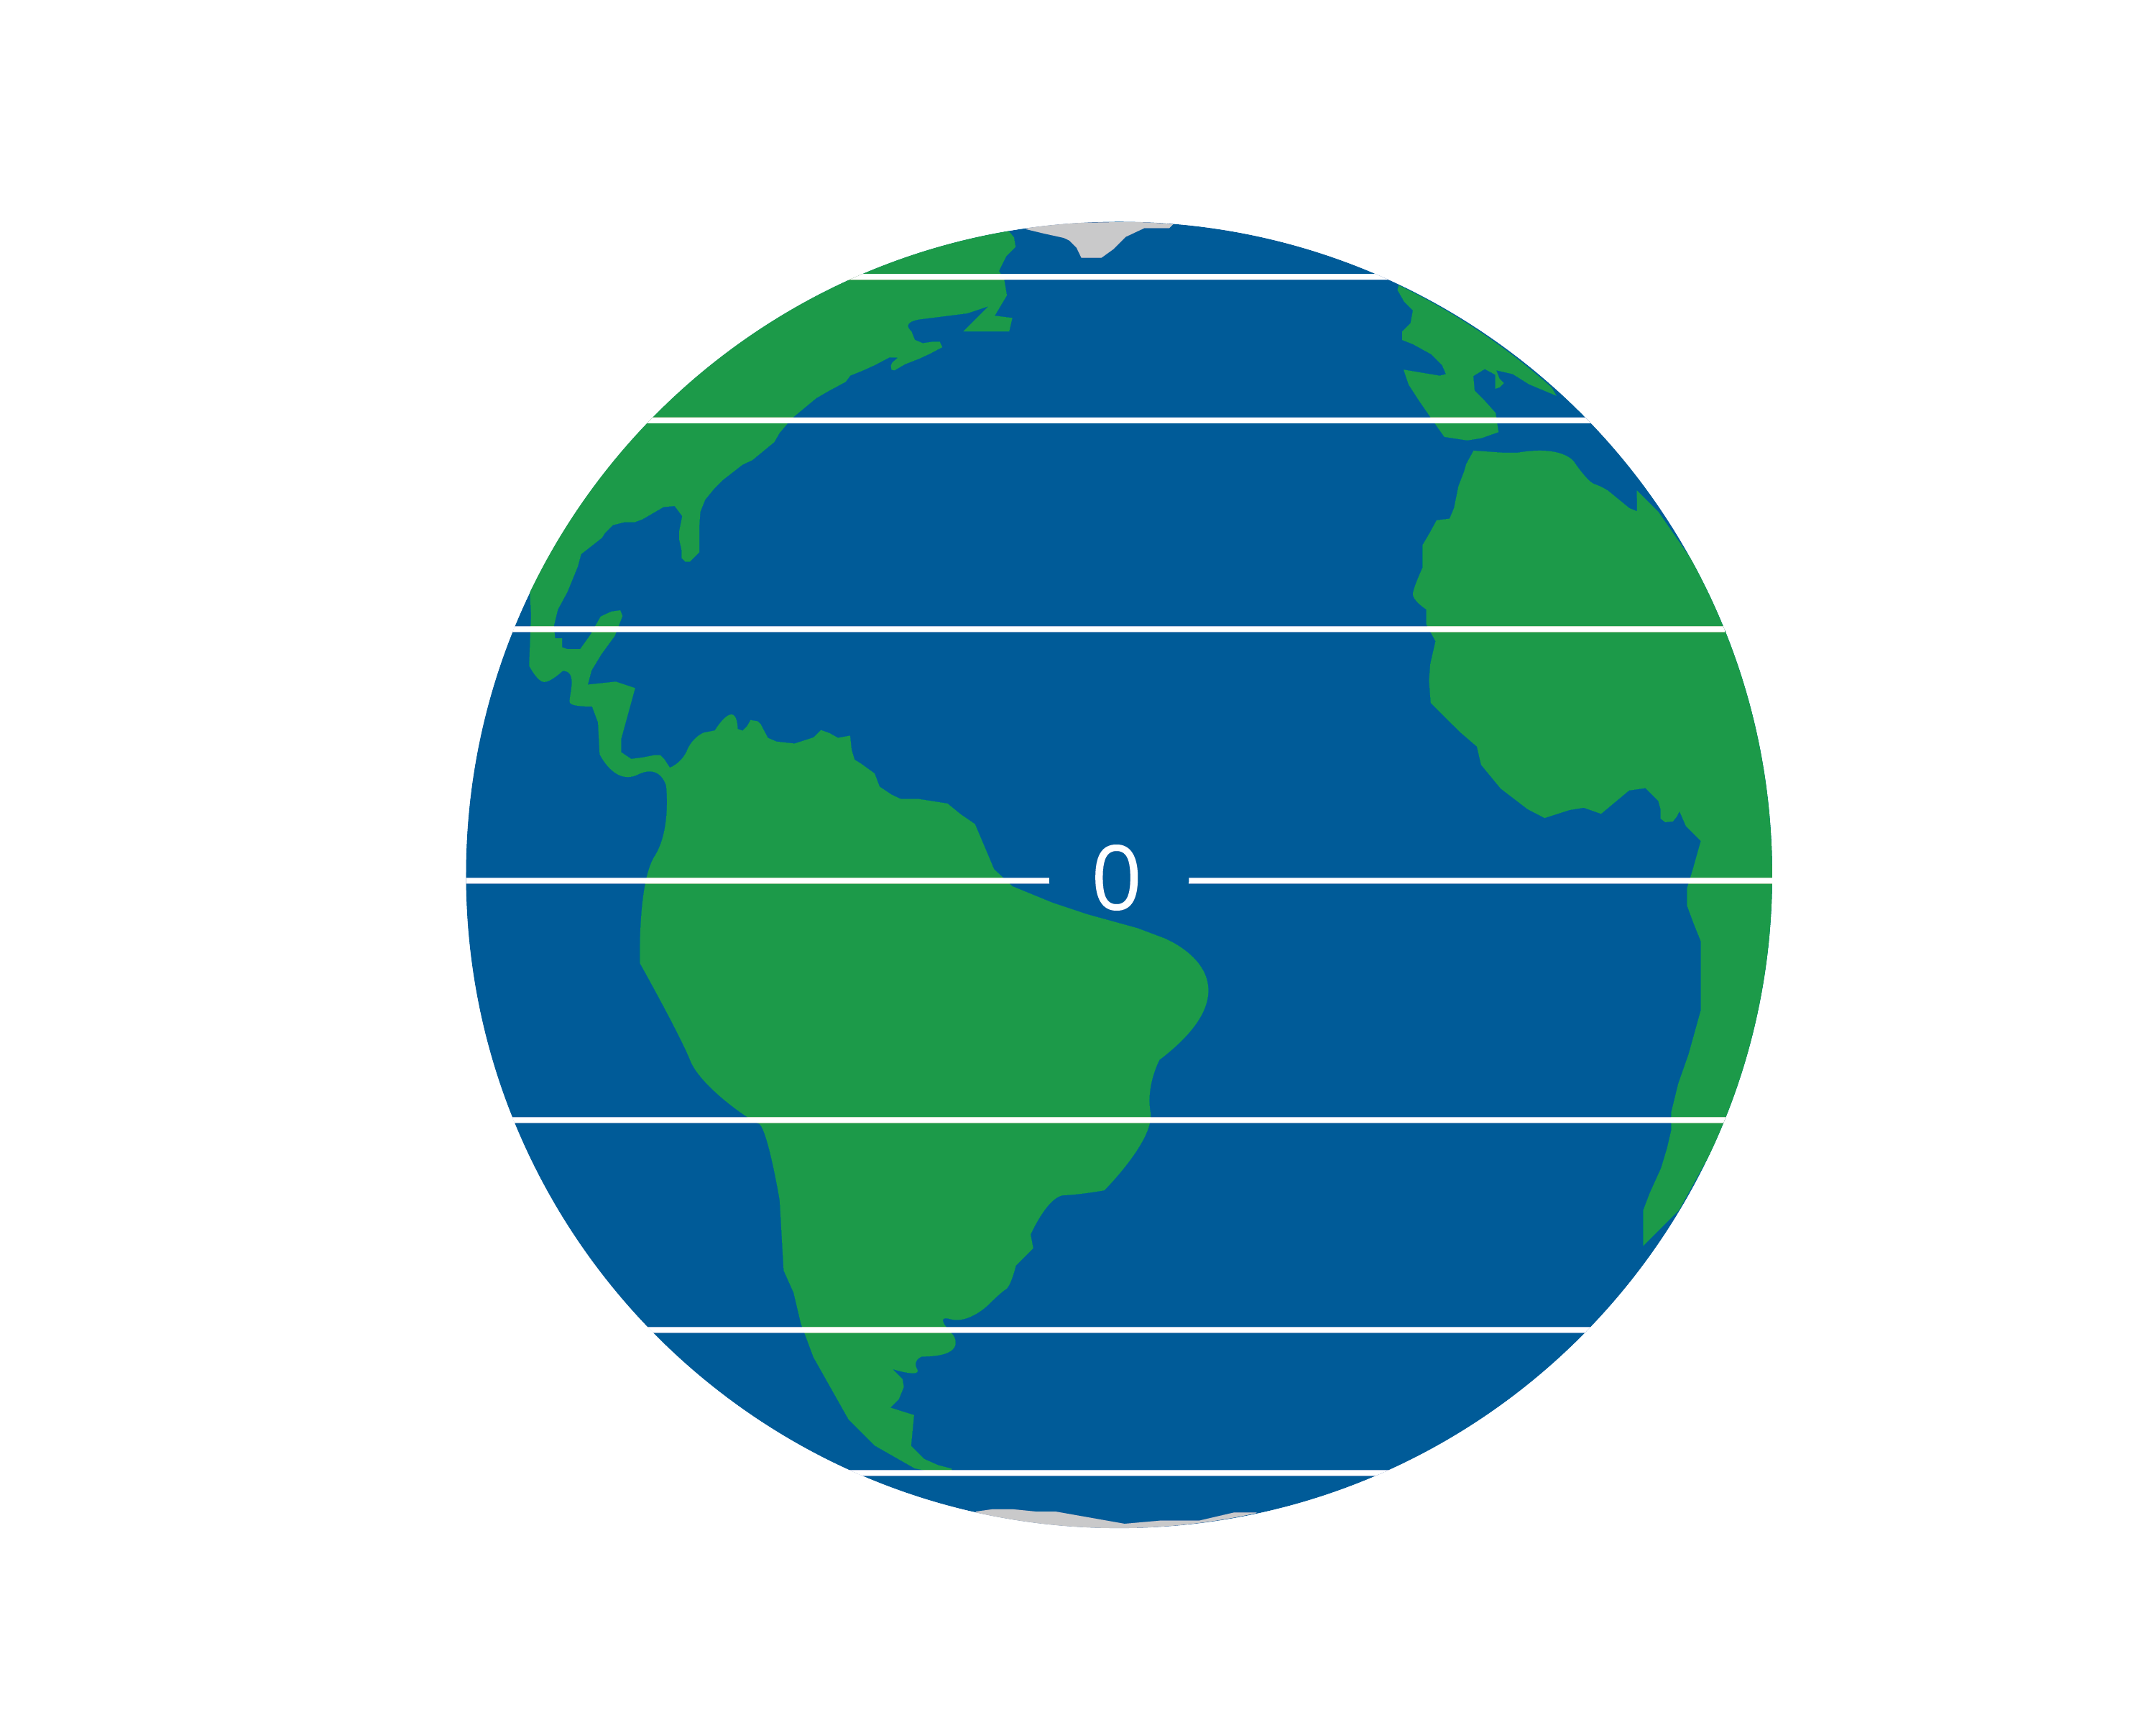
\includegraphics[width=.75\textwidth]{lat.png}
  \caption{Latitude drawn on the earth.}
  \label{fig:latitude}
\end{figure}

\begin{figure}[htbp]
  \centering
  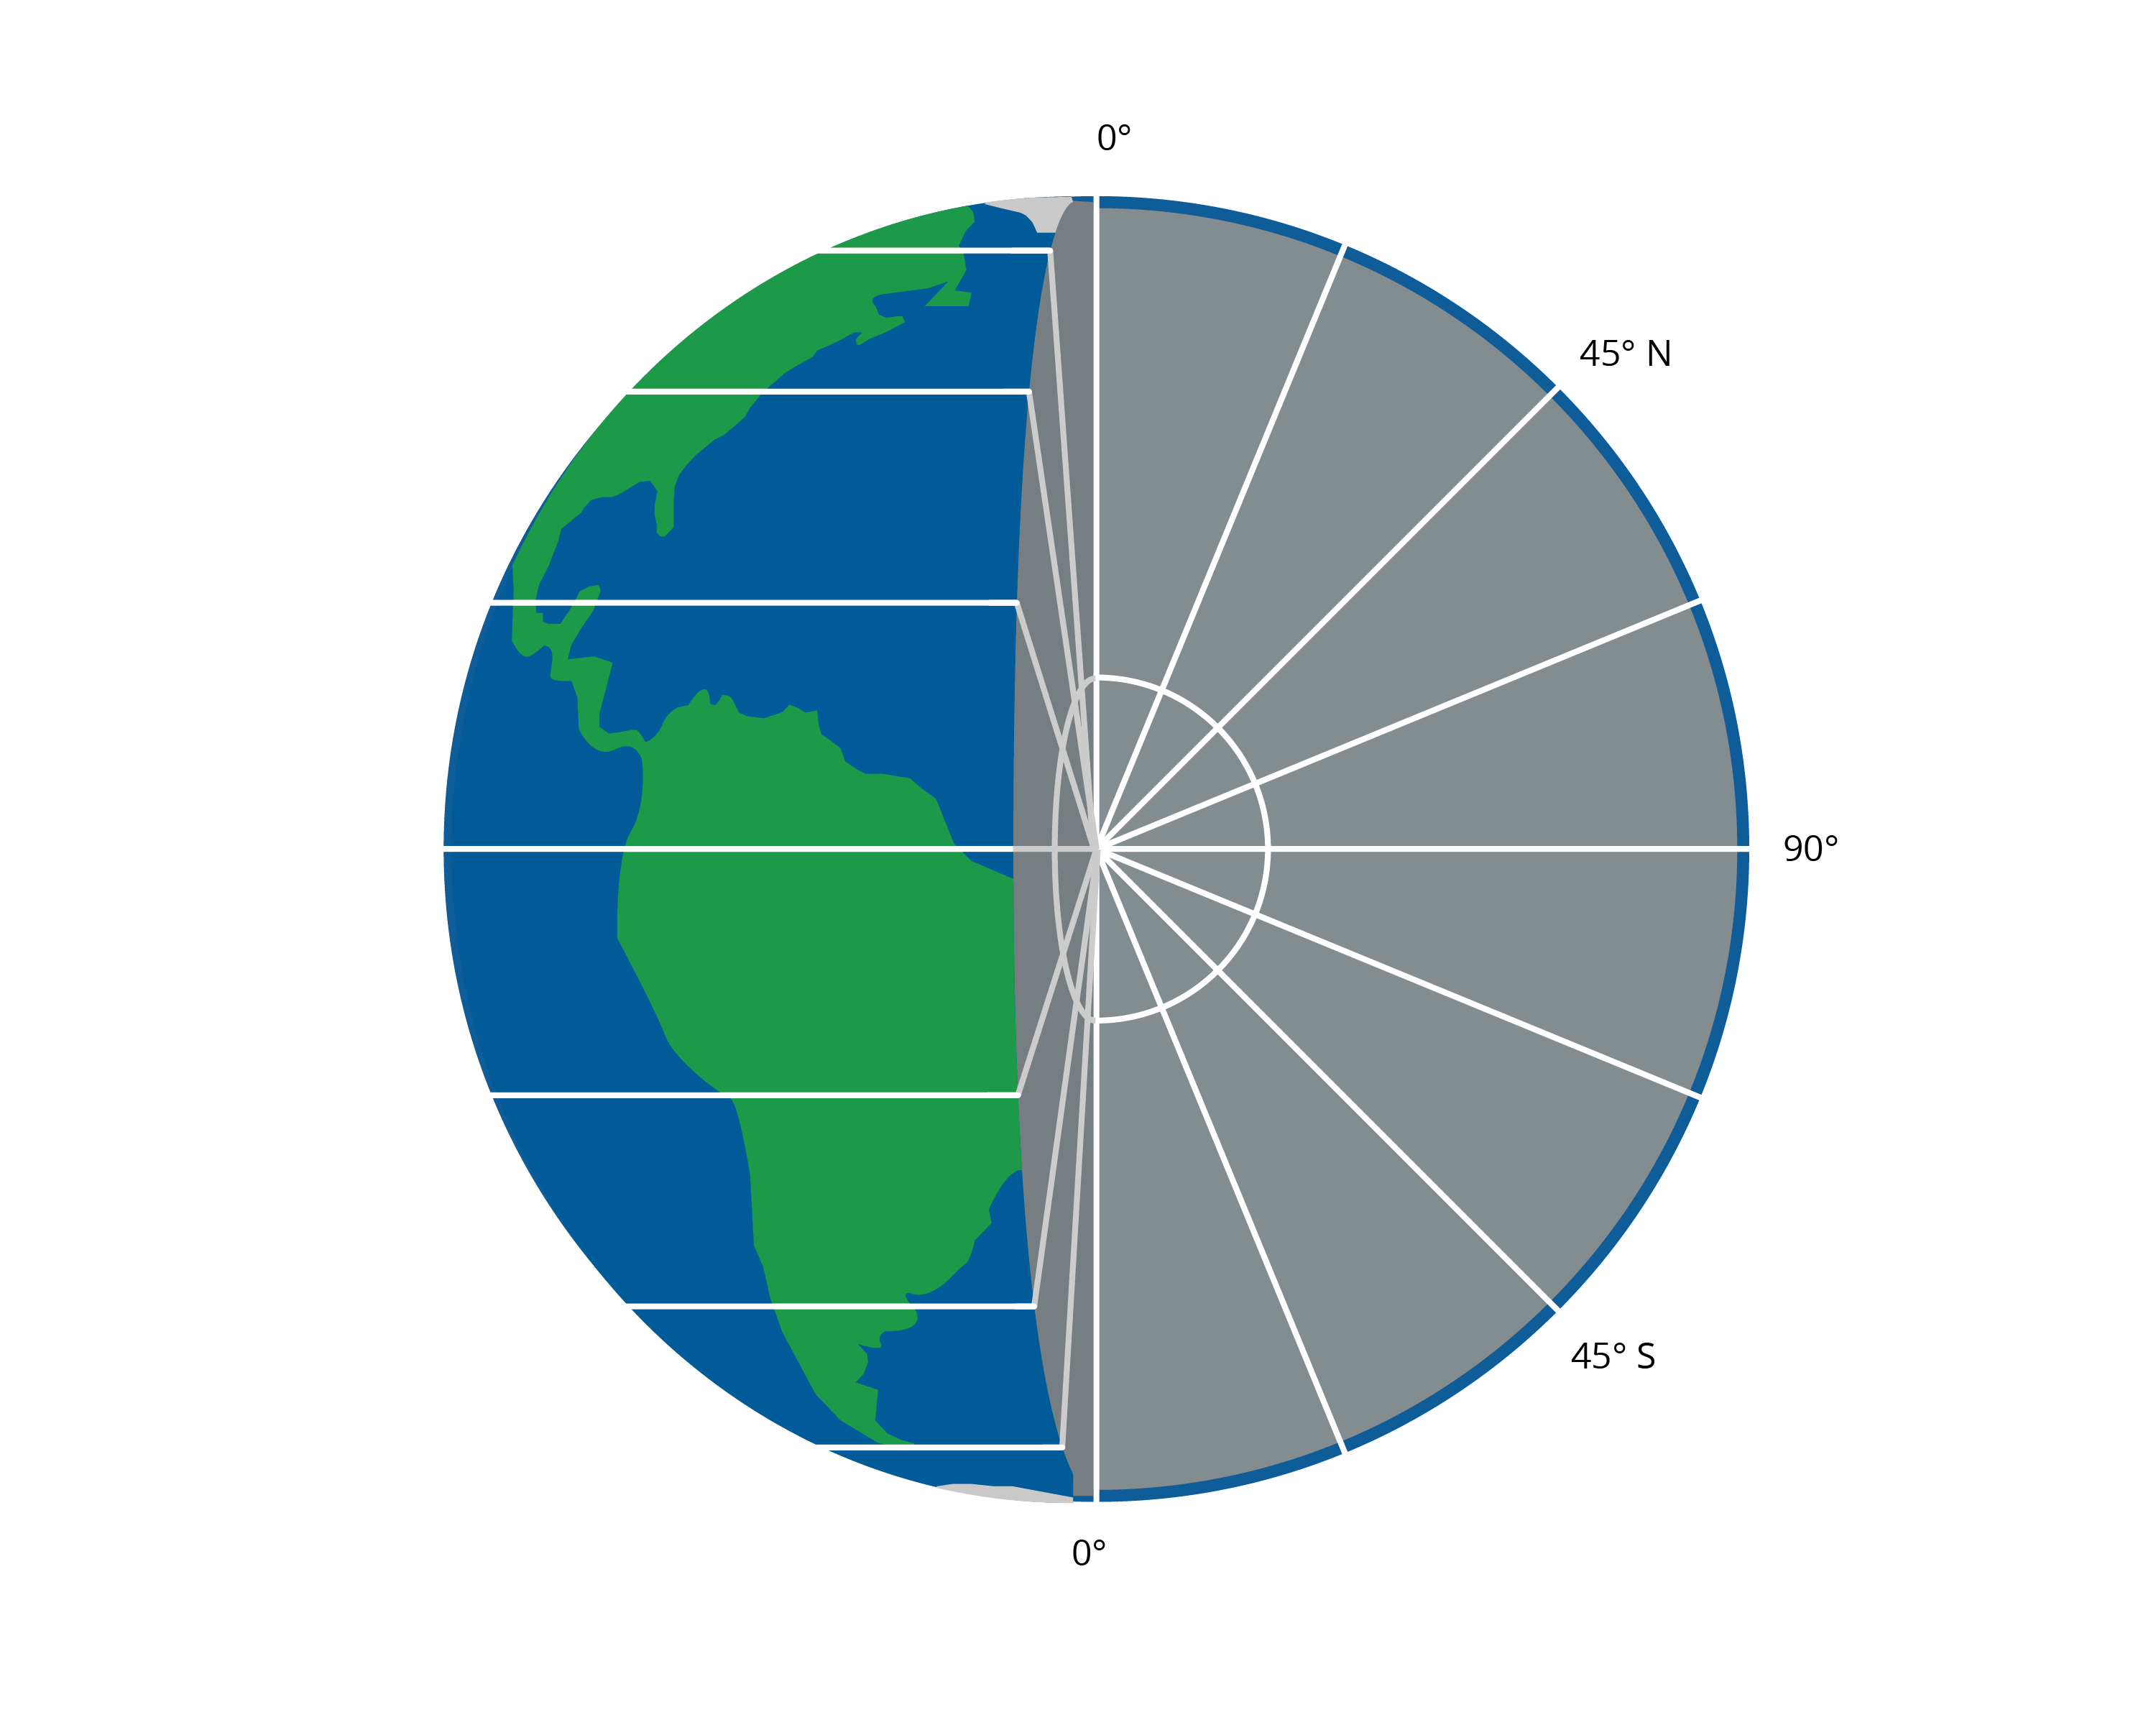
\includegraphics[width=.75\textwidth]{latExplanation.png}
  \caption{A cross-section of the earth showing latitude.}
  \label{fig:latitudeExplained}
\end{figure}
\index{longitude}
Longitude, on the other hand, measures a point's distance east or west
of the Prime Meridian (which passes through Greenwich, England). It
ranges from $-180^{\circ}$ to $+180^{\circ}$, with the Prime Meridian
represented as $0^{\circ}$. (See figures~\ref{fig:longitude} and~\ref{fig:longExplanation})

\begin{figure}[htbp]
    \centering
    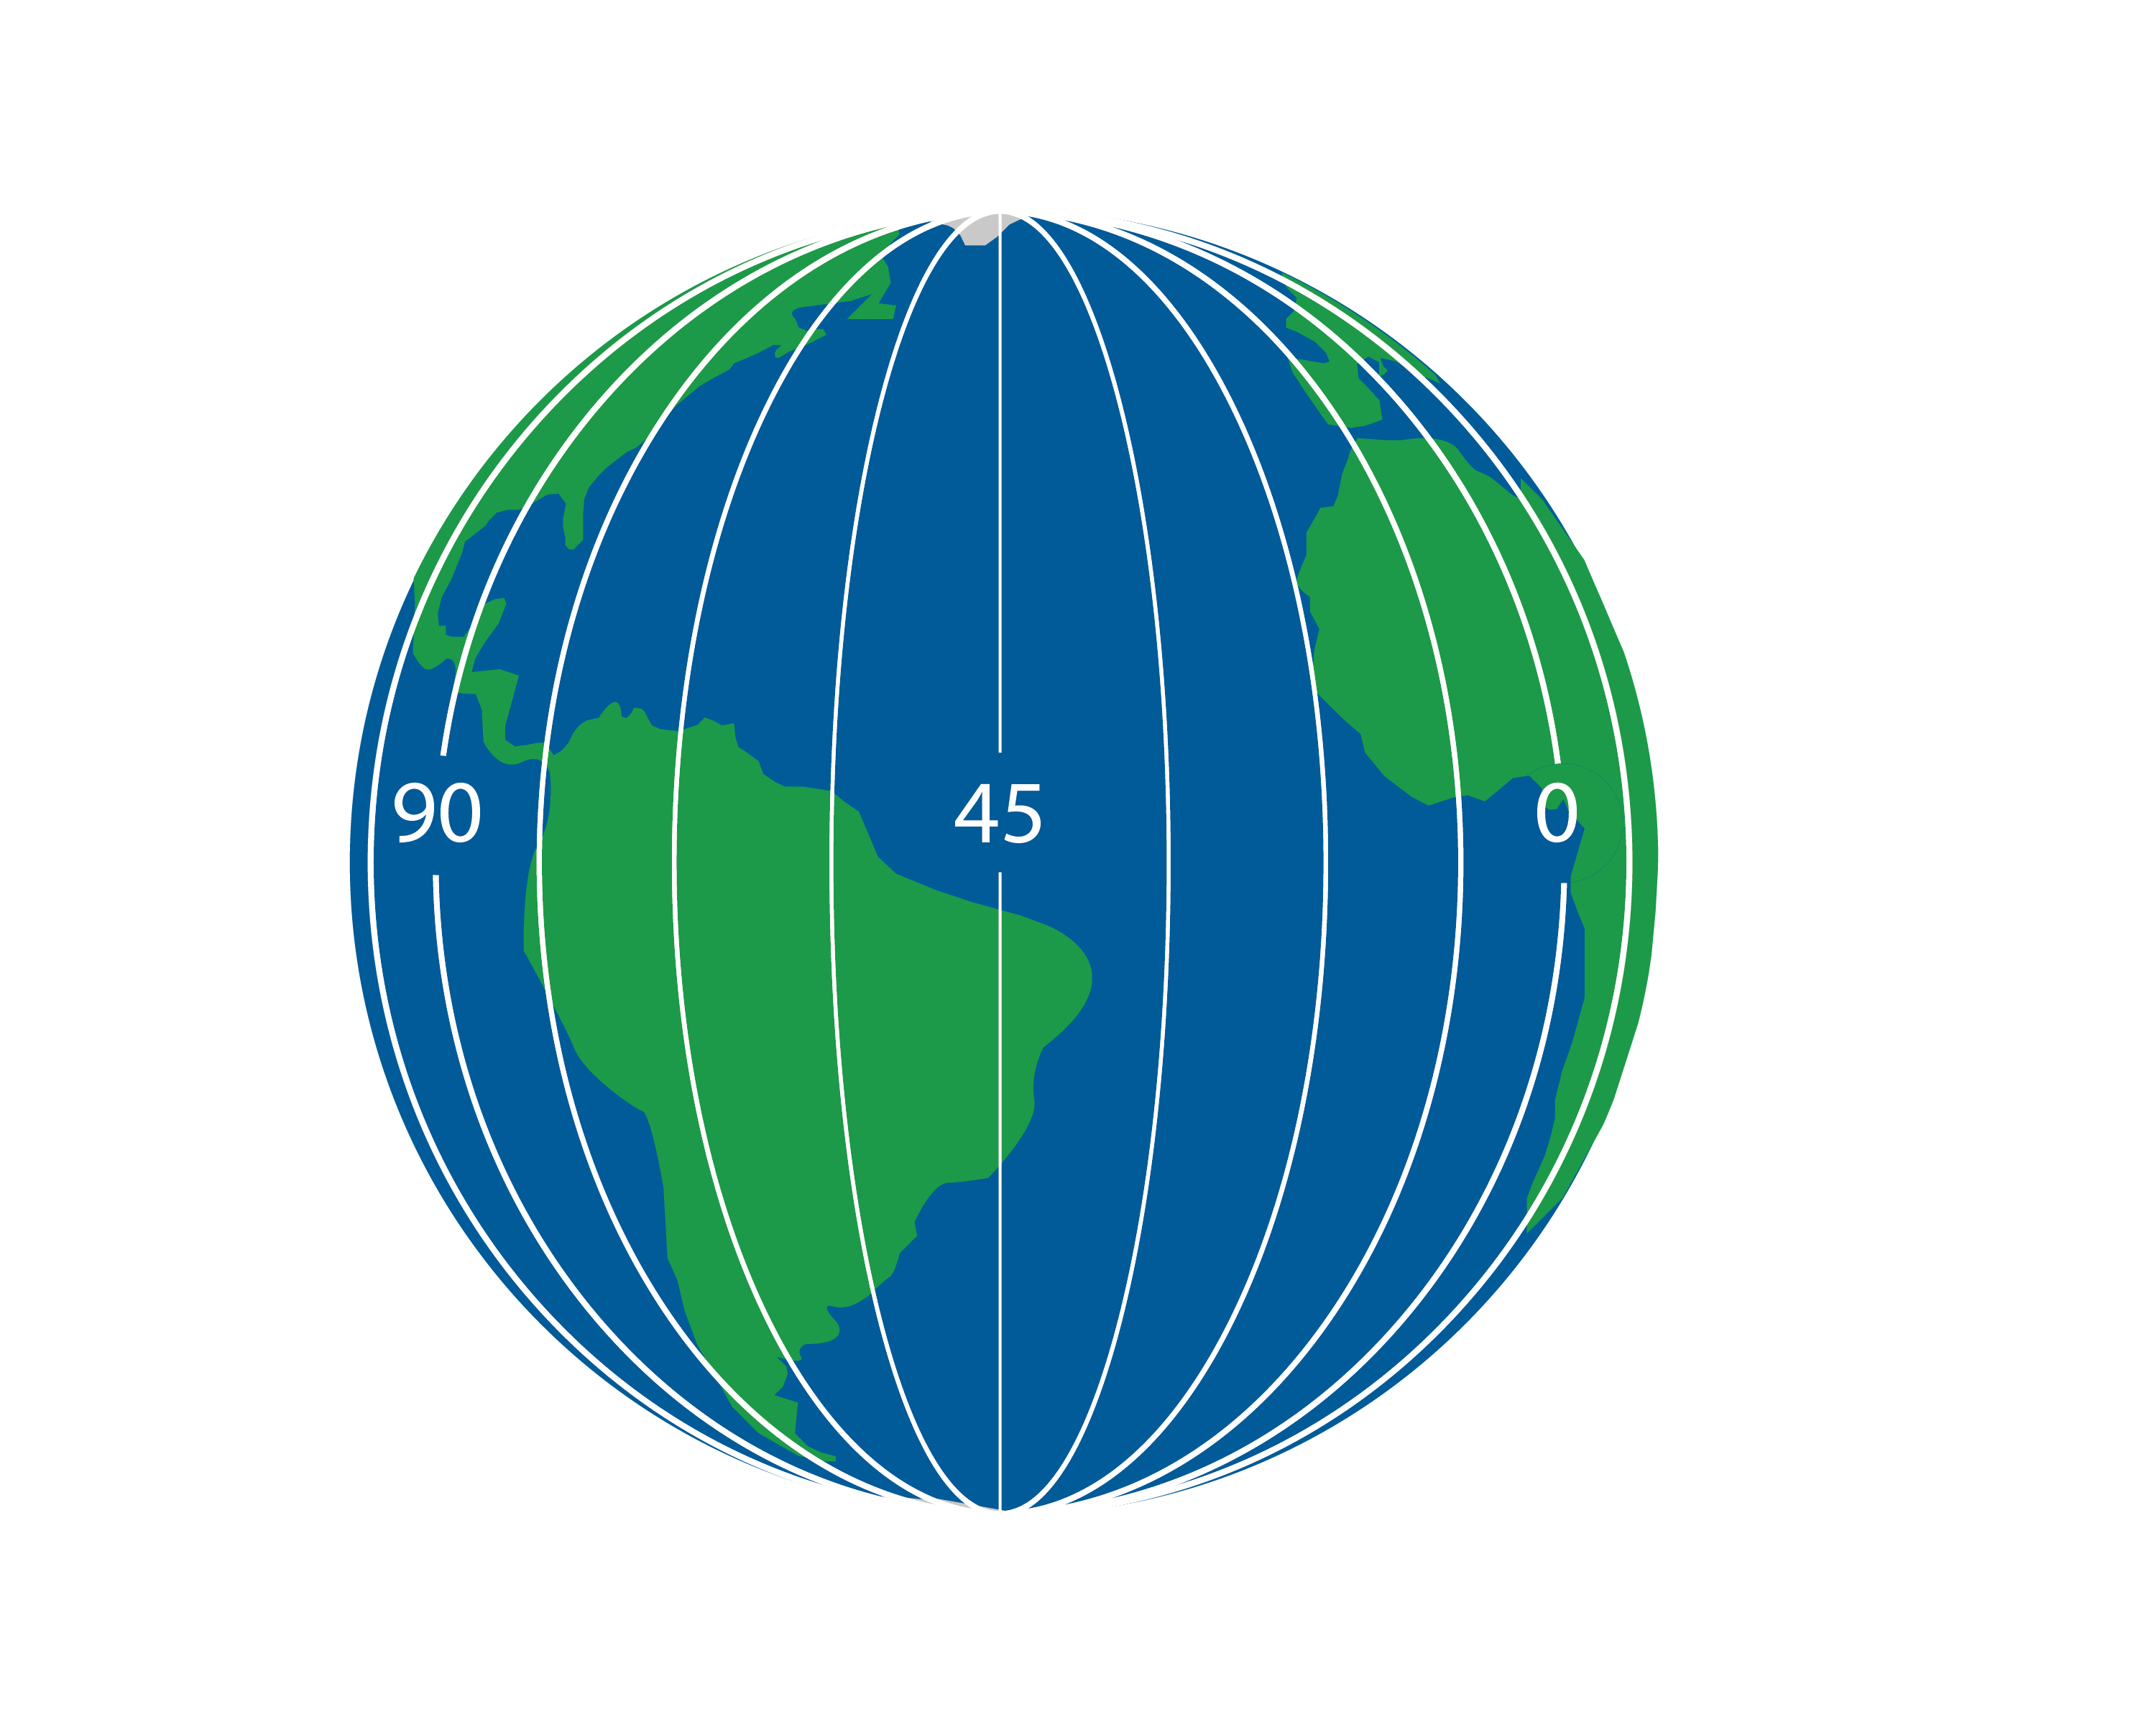
\includegraphics[width=.75\textwidth]{long.png}
    \caption{Longitudinal lines drawn on the earth.}
    \label{fig:longitude}
\end{figure}
\begin{figure}[htbp]
  \centering
  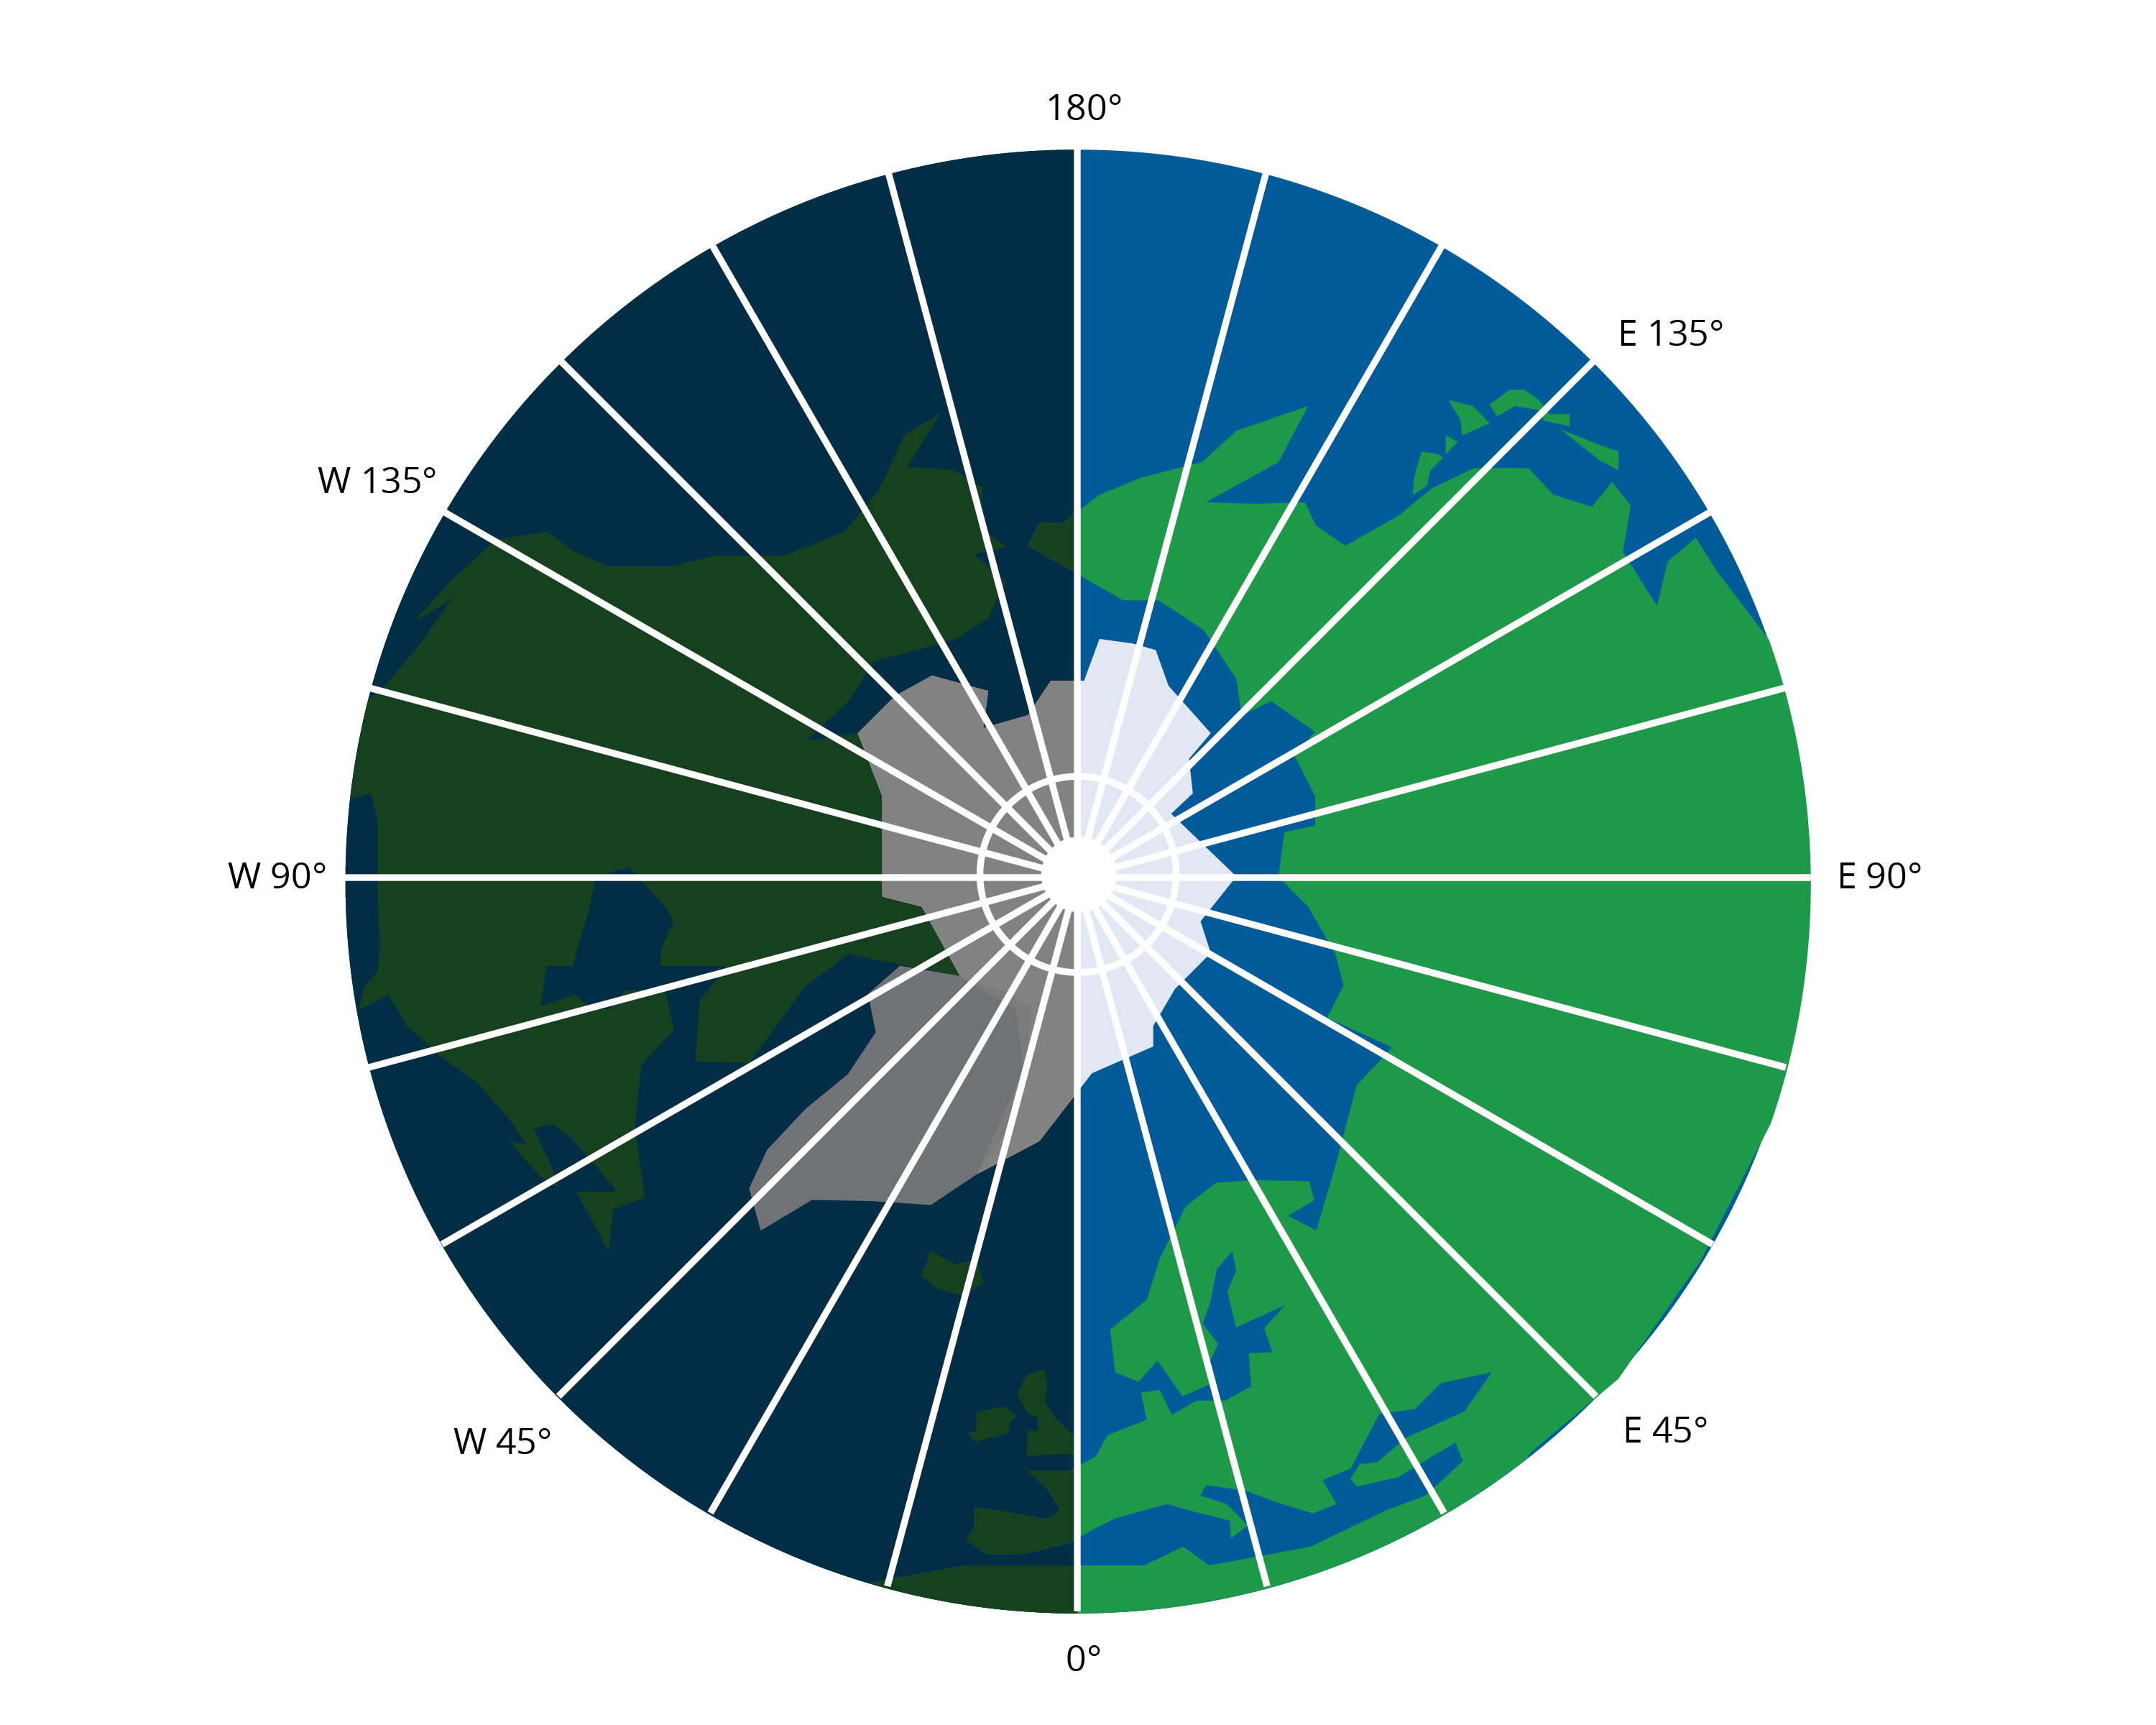
\includegraphics[width=.75\textwidth]{longExplanation.png}
    \caption{A cross-section of the earth showing longitude.}
    \label{fig:longExplanation}
\end{figure}
\index{Longitude and Latitude ! coordinates of}
The coordinates follow a system of latitude and then longitude (in the majority of contexts). Here is the Longitude and Latitude of four different large cities:
\begin{itemize}
  \item \textbf{London, England}: $51^\circ$ N $0^\circ$ W
  \item \textbf{New York City, New York, USA}: $40^\circ$ N $74^\circ$ W
  \item \textbf{Sydney, New South Whales, Australia}: $33^\circ$ S $150^\circ$ E
  \item \textbf{Rio de Janerio, Brazil}: $22^\circ$ S $43^\circ$ W
\end{itemize}

These coordinates may be broken down further into minute and second components as well, for futher geometric accuracy.
Each degree ($^\circ$) is divided into 60 minutes ($'$). Each minute ($'$) is divided into 60 seconds ($"$). Just like in time. Note some do not

\begin{itemize}
  \item \textbf{London, England}: $51^\circ$ 30` 26" N $0^\circ$ 7` 39" W
  \item \textbf{New York City, New York, USA}: $40^\circ$ 42` 46" N $74^\circ$ 0` 22" W
  \item \textbf{Sydney, New South Whales, Australia}: $33^\circ$ 52` 0" S $150^\circ$ 12` 0" E
  \item \textbf{Rio de Janerio, Brazil}: $22^\circ$ 54` 0" S $43^\circ$ 12` 0" W
\end{itemize}

\section{Nautical Mile}
\index{Nautical Mile}
A nautical mile is a unit of measurement used primarily in aviation
and maritime contexts. It is based on the circumference of the Earth,
and is defined as one minute ($1/60^{\circ}$) of latitude; in other words, \textbf{one minute of latitude is equal to 1 nautical mile.} 
This makes it directly related to the Earth's geometry, unlike a kilometer or a
mile, which are arbitrary in nature. The exact value of a nautical
mile can vary slightly depending on which type of latitude you use
(e.g., geodetic, geocentric, etc.), but for practical purposes, it is
often approximated as 1.852 kilometers or 1.15078 statute miles.\index{nautical mile}

\section{Haversine Formula}

The haversine formula is an important equation in navigation for
giving great-circle distances between two points on a sphere from
their longitudes and latitudes. It is especially useful when it comes
to calculating distances between points on the surface of the Earth,
which we represent as a sphere for simplicity. See Figure~\ref{fig:haversine} \index{Haversine formula}

\begin{figure}[htbp]
    \centering
    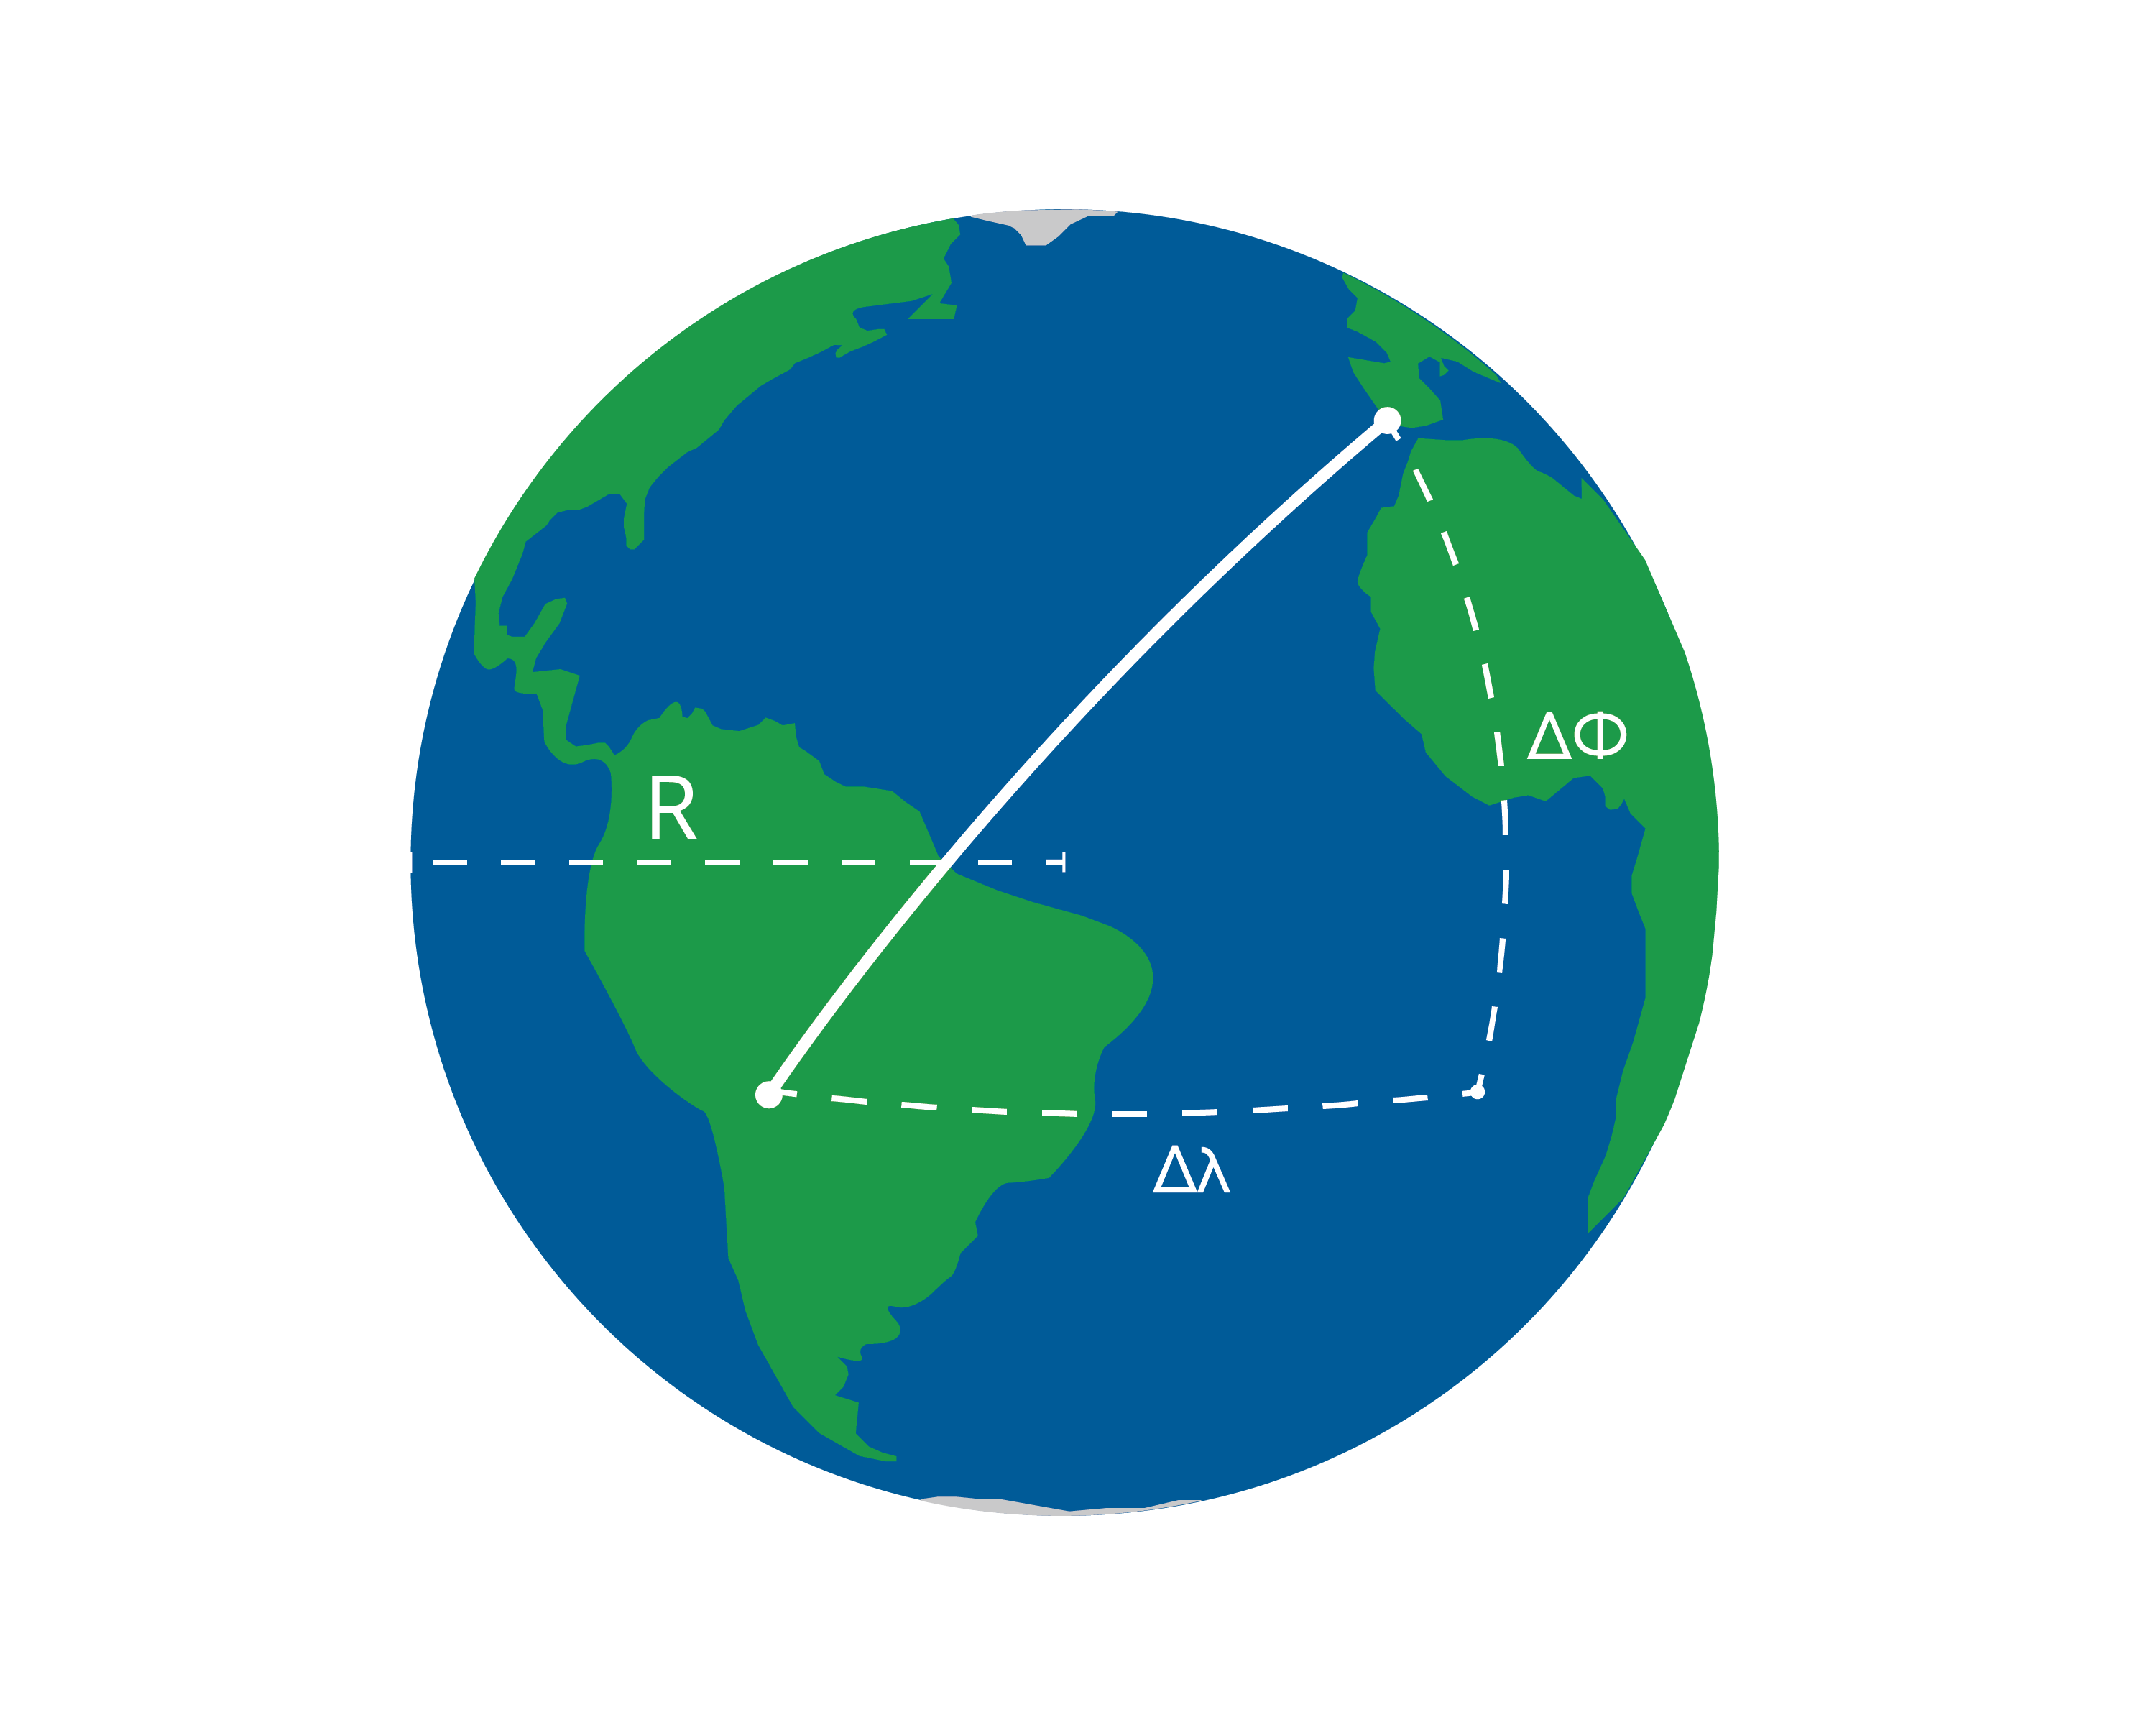
\includegraphics[width=\textwidth]{haversine.png}
    \caption{A diagram of the haversine formula.}
    \label{fig:haversine}
\end{figure}


In its basic form, the haversine formula is as follows:
%FIXME I feel like this section may need more clarification if the formula is important.

The angle found using haversine $\text{haversine}(\theta) = sin^2\left(\frac{\theta}{2}\right)$:

\[
a = \sin^2\left(\frac{\Delta\phi}{2}\right) + \cos(\phi_1)\cos(\phi_2)\sin^2\left(\frac{\Delta\lambda}{2}\right)
\]

Compute $c$ which determines the angular distance using $atan2$, a computer science tangential function with 2 arguments equivalent to $2 \arcsin(\sqrt{a})$\footnote{Note that this function is not available on calculators, but commonly used in computer science programs. You may use the singular argument equivalent in calculations.}:
\[
c = 2 \cdot \text{atan2} \left( \sqrt{a}, \sqrt{1-a} \right)
\]


Find $d$, the true distance along the sphere:

\[
d = R \cdot c
\]

In one line, this is:
$$
d = 2R \cdot \arcsin\left( \sqrt{\sin^2\left(\frac{\Delta\phi}{2}\right) + \cos(\phi_1) \cos(\phi_2) \sin^2\left(\frac{\Delta\lambda}{2}\right)} \right)
$$

Here, $\phi_1$ and $\phi_2$ represent the latitudes of the two points (in radians),
$\Delta\phi$ and $\Delta\lambda$ represent the differences in latitude
and longitude (also in radians), and $R$ is the radius of the
Earth (using whatever unit of distance you desire). The result, $d$, is the distance between the two points along
the surface of the sphere. Notice that $d$ is equal to the formula for the \emph{arc length} of a sector. 
A sphere is just a bunch of circles with radius $r$, so it follows that we can use formulas for circles in our spherical calculations. 

This is why planes fly arc-shaped paths rather than straight paths from points $A \to B$. Planes follow the shortest path between two points on a sphere, called a \emph{great-circle route}. On a map, like plane flight-progress maps or the Mercator projection, the straight path looks very arc shaped, but this is just a geographical illusion. This straight distance can be calculated using the haversine formula, ultiamtely minimizing distance and fuel using the `as-the-crow-flies' path. 


\graphicspath{{../../Chapters/geocoding/en_US}}
\chapter{Geocoding and Reverse Geocoding}

Geocoding and reverse geocoding are essential processes in geographic
information systems (GIS) that are used to convert between addresses
and spatial data.

\section{Geocoding}

Geocoding is the process of converting addresses (like "1600
Amphitheatre Parkway, Mountain View, CA") into geographic coordinates
(like latitude 37.423021 and longitude -122.083739), which you can use
to place markers on a map, or position the map. The resulting latitude
and longitude are often used as a key index in merging datasets based
on location.\index{geocoding}

Here is an example of using Google's Geocoding service to get the
longitude and latitude of the Dallas County Administration Building:

\begin{verbatim}

import requests
import json

# Encode the parameters
parameters = {"address": "411 Elm St, Dallas, TX 75202", "key": "YOUR_API_KEY"}
base_url = "https://maps.googleapis.com/maps/api/geocode/json?"

# Send the GET request
response = requests.get(base_url,  params=parameters)

# Convert the response to json
data = response.json()

# Extract the latitude and longitude
if len(data["results"]) > 0:
    latitude = data["results"][0]["geometry"]["location"]["lat"]
    longitude = data["results"][0]["geometry"]["location"]["lng"]
    print(latitude, longitude)
else:
    print(f"Could not find the latitude and longitude .")
    
\end{verbatim}

\section{Reverse Geocoding}

Reverse geocoding, as the name implies, is the opposite process of
geocoding. It involves converting geographic coordinates into a
human-readable address. This can be useful in applications where you
need to display an actual address to a user instead of latitude and
longitude coordinates.\index{reverse geocoding}

Here is an example of using Google's reverse geocoding API\footnote{Note that the API key is something you obtain on your own, people do not share API keys for privacy and security reasons.} to find the
address at latitude = 33.9474096, longitude = -118.1179069


\begin{verbatim}
import requests
import json

api_key = "YOUR_API_KEY"
latitude = 33.9474096
longitude = -118.1179069

    # Encode the parameters
parameters = {"latlng": f"{latitude},{longitude}", "key": api_key}
base_url = "https://maps.googleapis.com/maps/api/geocode/json?"

# Send the GET request
response = requests.get(base_url, params=parameters)

# Convert the response to json
data = response.json()

# Extract the address
if len(data["results"]) > 0:
    address = data["results"][0]["formatted_address"]
    print(address)
else:
    print(f"Could not find the address")

\end{verbatim}
\graphicspath{{../../Chapters/making_a_map/en_US}}
\chapter{Making a Map}


Plotly is an open-source data visualization library for Python, R, and JavaScript. It allows for interactive plots, including geographical maps. In this brief example, we will learn how to create a simple annotated map using Plotly in Python.

To start, you need to install Plotly. In Python, you can do this via pip:

\begin{lstlisting}[language=Python]
pip install plotly
\end{lstlisting}

Once installed, you can create a map with annotations as follows:

\begin{lstlisting}[language=Python]
import plotly.graph_objects as go

fig = go.Figure(data=go.Scattergeo(
    lon = [-75.789], 
    lat = [45.4215],
    text = ['Ottawa'],
    mode = 'text',
))

fig.update_layout(
    title_text = 'Annotated Map with Plotly',
    showlegend = False,
    geo = dict(
        scope = 'world',
        projection_type = 'azimuthal equal area',
        showland = True,
        landcolor = 'rgb(243, 243, 243)',
        countrycolor = 'rgb(204, 204, 204)',
    ),
)

fig.show()
\end{lstlisting}

This code creates a world map and places a text annotation at the geographic coordinates for Ottawa. The `go.Scattergeo` function is used to define the geographical scatter plot (i.e., the annotation), while the `update\_layout` function is used to define the appearance and the properties of the map itself.

In this example, you can replace the latitude, longitude, and text with the values corresponding to your desired location.

%%%%%%%%%%%%%%%%%%%%%%%%%%%%%%%%%
%% Bookfooter.tex by Aaron Hillegass
%% Nov 8, 2020

\appendix

\chapter{Answers to Exercises}
\shipoutAnswer

\bibliography{references}

\printindex

\end{document}